\paragraph{Элементы информационной модели}

Каждая сущность в проекте информационной модели называется элементом.
Revit использует 3 типа элементов в проектах:
элементы модели, опорные элементы и элементы, относящиеся к представлению.
Элементы в Revit также часто называются семействами.
Семейство содержит геометрическое определение элемента и
параметры, используемые элементом.
Каждый экземпляр элемента определяется и контролируется семейством.%
\cite{DocRevit}
Для создания визуализации нас в первую очередь интересуют
именно элементы модели.

\begin{figure}[ht]
    \centering
    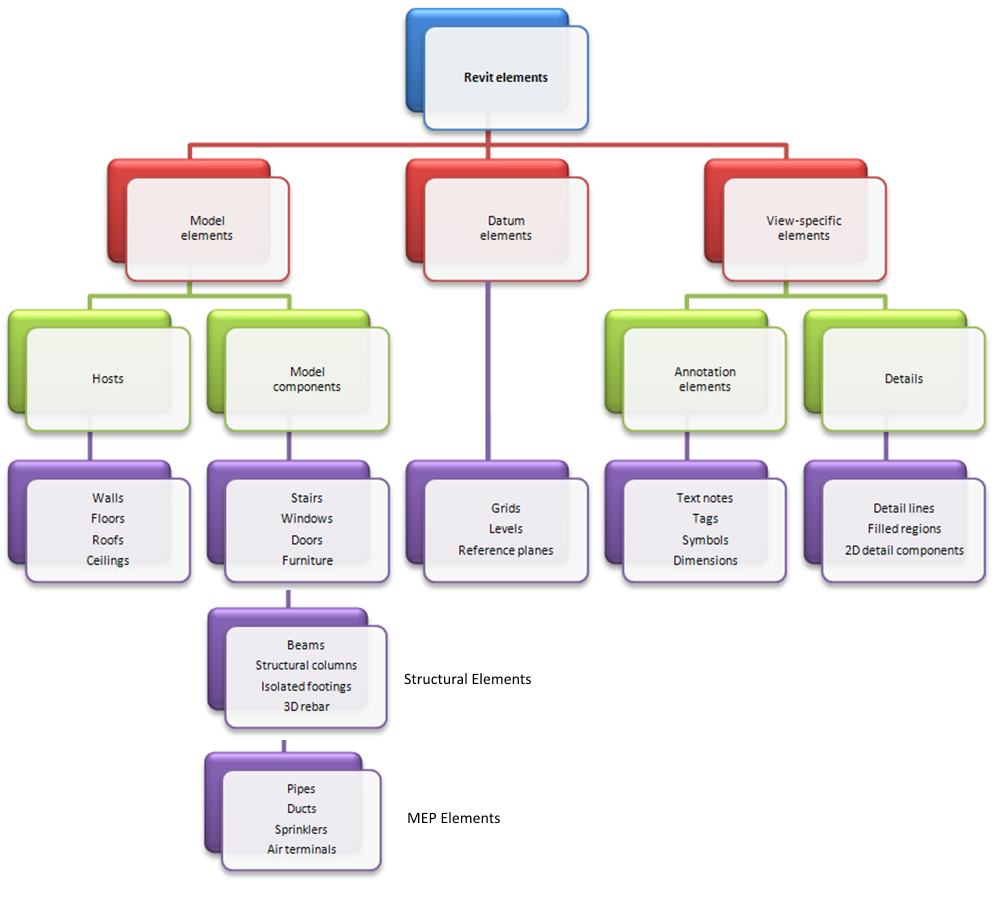
\includegraphics[width=0.9\textwidth]{images/Revit-elements.png}
    \caption{Элементы информационной модели.%
    \cite{DocRevit}}
    \label{figure:RevitElements}
\end{figure}

\begin{itemize}
    \item {
        Элементы модели.

        Элементы модели представляют фактическую трехмерную геометрию здания,
        например стены, окна, двери, пандусы,
        воздуховоды и электрические панели.
        Элементы модели делятся на хосты и компоненты модели.
        Хостами обычно являются элементы,
        которые возводятся непосредственно на строительной площадке,
        например стены и потолки.
        Компонентами модели являются все остальные типы элементов модели.
    }
    \item {
        Опорные элементы.

        Опорные элементы помогают определить контекст проекта.
        К ним относятся опорные плоскости, уровни и сетки.
    }
    \item {
        Элементы представления.

        Элементы представления это элементы,
        отображаемые только в каком-то определенном режиме представления проекта.
        Они помогают описывать или документировать модель.
    }
\end{itemize}
